\chapter{Background}
\label{chap:background}
\section{Distributed Hash Tables}
\label{sec:background_dhts}
Distributed hash tables (DHTs) are a method of distributing data storage to
nodes in a network. From an abstract point of view, they are just hash tables
that map keys to values. They are appealing because they offer robust data
storage without the need for a central authority.

The keys usually have fixed length, the values, or records, can be arbitrary
data. Some care should be taken to ensure there are no collisions in keys. Using
a cryptographic hash of the record itself is a useful way of achieving that for
DHTs storing files. For a DHT storing reachability information of peers like in
this thesis, using the unique ID of the peers makes sense.

Each node in the DHT stores a number of the records. In the language of this
thesis, it is \emph{responsible for} them. The key of a record determines who is
responsible for it, and there is a distance metric measuring how far a node is
to being responsible for a record. In the DHT used in this thesis every node has
an ID that has the same format as the keys in the DHT. A node is responsible for
a record if its key has the same prefix as its own ID.

A node in the network doesn't need to know all other nodes, but for any key it
must know another node closer to that node. Then it is possible to route to any
record stored in the DHT. The node can ask the closer node for the record, which
in turn asks another node closer, eventually reaching a responsible node.

Node IDs and which records nodes are responsible for can be illustrated on a
binary tree. Figure~\ref{fig:node_id_tree} does this. Following the path from
the root node to a node (left being \texttt{0}, right \texttt{1}) yields a
prefix of the node's ID. This is also the prefix of the keys the node is
responsible for. Finding a node closer to a key is done by moving up the tree
towards the root, then descending once the path matches the key.

Records can be created, updated and deleted by contacting the node responsible
for the corresponding key.

A useful robustness feature is replication, in which more than one node is
responsible for each record. This way, if a node fails, the record is not lost.
All the nodes responsible for the same records must stay in contact to
synchronize their records, making each other aware of new and updated records as
well as deletions.

Load balancing is another advanced feature that's useful if some records are
much more popular, or much bigger than others. To achieve it, the mapping from
node to the records the node is responsible for must be mutable. More nodes are
then made responsible for the records that generate a lot of traffic.

\begin{figure}[t]
  \centering
  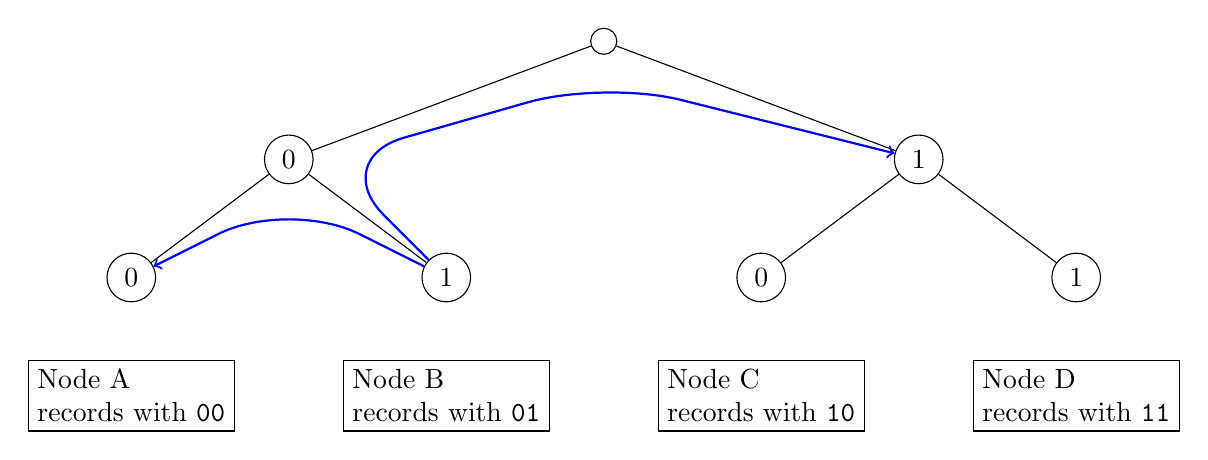
\begin{tikzpicture}
    \begin{scope}[every node/.style={circle, draw}]
      \node (0) at (0, 0) {};
      \node (10) at (-4, -1.5) {0};
      \node (11) at (4, -1.5) {1};
      \node (20) at (-6, -3) {0};
      \node (21) at (-2, -3) {1};
      \node (22) at (2, -3) {0};
      \node (23) at (6, -3) {1};
    \end{scope}
    \begin{scope}[every node/.style={rectangle, draw, align=left}]
      \node (A) at (-6, -4.5) {Node A\\records with \texttt{00}};
      \node (B) at (-2, -4.5) {Node B\\records with \texttt{01}};
      \node (C) at (2, -4.5) {Node C\\records with \texttt{10}};
      \node (D) at (6, -4.5) {Node D\\records with \texttt{11}};
    \end{scope}

    \draw (0) -- (10);
    \draw (0) -- (11);
    \draw (10) -- (20);
    \draw (10) -- (21);
    \draw (11) -- (22);
    \draw (11) -- (23);
    \draw[rounded corners=10mm, ->, thick, color=blue] (21) -- (-3.5, -1.5)
        -- (0, -0.5) -- (11);
    \draw[rounded corners=10mm, ->, thick, color=blue] (21) -- (-4, -2) -- (20);
  \end{tikzpicture}
  \caption{The responsibilities of nodes can be illustrated on a tree. Node A
  stores all records whose key begins with \texttt{00}, node B all those with
  \texttt{01} etc. When a node needs a record he doesn't store himself, he needs
  to ask someone else. He finds the right node to ask by going up in the tree
  until the path in the tree matches the key, then descending down the other
  side.  For example, if node B needs a record starting with \texttt{00}, he
  asks node A, if he needs a record starting with \texttt{1}, he asks either
  node C or node D (blue arrows).}
  \label{fig:node_id_tree}
\end{figure}

\section{Discrete Event Simulation}
A discrete event simulation framework simulates a system by processing events at
discrete times. This can be implemented deterministically, making the
simulations reproducible.

In execution, the framework maintains the current
\emph{simulated time}, i.e. the time within the simulation, which counts up as
the simulation progresses. The central part of the framework is the event queue,
which contains events, each together with the time at which it should be
triggered.

An event is the unit of action in the framework and models something taking
place. This can for example be a message being sent over the network. Events can
be \emph{triggered}, meaning the action they represent is executed. They can
then mutate the state of the system, as well as place new events on the event
queue. For example, the message-sent event could modify the sender's state for
outbound messages and place a message-received event in the event queue a little
bit in the future.

The simulation is initialized by placing at least one event in the queue. When
it is started, the framework continually pops the next event (the one with the
lowest trigger time) from the event queue, forwards the simulated time to the
event's trigger time, and triggers the event.

If the last event taken from the queue doesn't place any new events, the
simulation ends. But there are also other useful termination criteria, like
reaching a (wall clock) time limit, reaching a simulated time limit, or e.g.
reaching a certain number of events processed.

The procedure described is serial, i.e. single-threaded. Discrete event
simulations can be parallelized, but this takes some effort. Race conditions can
occur if two successive events are removed from the event queue and triggered
concurrently. These must be detected, the system rolled back, and the events
processed again sequentially. This issue can be made less likely by distributing
events across threads such that events that are likely to cause race conditions
are processed in the same thread.

In this thesis, the SimPy framework~\cite{simpy} was used. It is written in
Python, allowing for quick iteration of the model. However, it can't be
parallelized, so the simulation is strictly single-threaded. Parallelizing was
considered difficult considering that the point of the system is that everyone
is able to spread out messages to a lot of other users. Thus, there would likely
not be clusters that could be assigned to one thread.

\section{Game Theory}
Game theory studies the interaction between rational actors within regulated
frameworks called games, and the dynamics emerging from it.

A game has a number of participants called players. Each player has a set of
possible behaviors, called strategies, that he must choose from to play the
game. The players choose their respective strategies simultaneously, i.e. no
player knows another player's strategy before picking his own strategy. The
vector of strategies picked by the players is called the outcome. Further, each
player has a utility function that maps every possible outcome to a value
denoting how desirable the outcome is for the player.

A game can be repeated, i.e. played in multiple rounds. After the game is played
for the first round, each player knows what strategies the other players picked.
The players can take this information into account when they pick their strategy
for the next round. They can also consider how their choice of strategy affects
other players' strategies in following rounds. E.g., a player may choose to
behave well towards other players so that they don't punish him in successive
rounds.

The terms \emph{cooperate} and \emph{defect} are commonly used. Cooperating with
others refers to player behavior that is generally well-behaved towards other
players, defecting on others in contrast means to let others down in some way.
In the context of this thesis, peers are behaving cooperatively if they play by
the rules, respond to queries etc., while peers are considered to be defecting
if they e.g. ignore incoming queries out of laziness.

The notion of equilibria is important in game theory. An equilibrium is a fixed
point in the behavior of the players, where all of them stick to their strategy.
More formally, an outcome is a pure Nash equilibrium if no player could increase
his utility in a future round given that all other players maintain their
strategy. The thinking is that each player tries to maximise his utility in the
next round and assumes that all other players will stick to their strategy.

In the reputation system proposed in this thesis, the behavior of peers can be
viewed as the behavior of players in a repeated game. The game would be played
within the query groups introduced in Section~\ref{sec:desc_query_groups}.
However, since there are many peers in those groups and they have many options
on how to behave, modeling their behavior formally is complicated. For this
reason, simulation is done instead.
